\documentclass[a4paper, 10pt]{article}

\usepackage[english,russian]{babel}
\usepackage[T2A]{fontenc}
\usepackage[utf8]{inputenc}
\usepackage{amsmath, amsfonts, amssymb, amsthm, mathtools}

\usepackage{indentfirst}
\usepackage{icomma}
\usepackage{hyperref}
\usepackage{soulutf8}
\usepackage{multirow}
\usepackage{hhline}
\usepackage{booktabs}
\usepackage{graphicx}

\usepackage{tikz}
\usepackage{wrapfig}
\usepackage{caption}
\usepackage{subcaption}

\usepackage{geometry}
\geometry{top=25mm}
\geometry{bottom=30mm}
\geometry{left=20mm}
\geometry{right=20mm}

\renewcommand{\epsilon}{\varepsilon}
\newcommand{\mean}[1]{\left<#1\right>}

\title{\textbf{Работа 1.3.1} \linebreak Определение модуля Юнга на основе исследования деформаций растяжения и изгиба}
\author{Константин Ерёмин Б03-204}
\date{Октябрь 2022}

\begin{document}
	\maketitle
	
	\section{Введение}
		\textbf{Цель:} экспериментально получить зависимость между напряжением и деформацией (закон Гука) для двух простейших напряжённых состояний упругих тел: одноосного растяжения и чистого изгиба; по результатам измерений вычислить модуль Юнга. \\
		
		\textbf{В работе используются:} в первой части --- прибор Лермантова, проволока из исследуемого материала, зрительная труба со шкалой, набор грузов, микрометр, рулетка; во второй части --- стойка для изгибания балки, индикатор для измерения величины прогиба, набор исследуемых стержней, грузы, линейка, штангенциркуль.
	
	\section{Предварительное описание работы}
	
		\begin{wrapfigure}{h}{0.3\textwidth}
			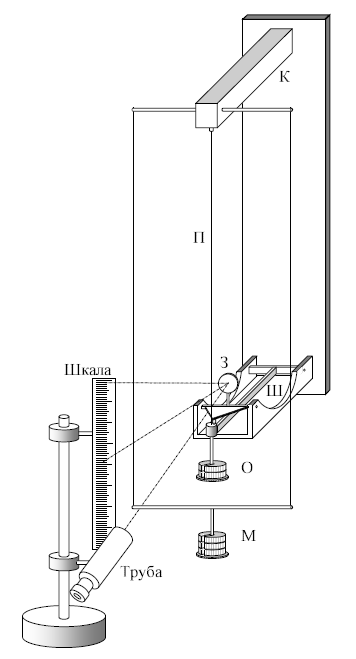
\includegraphics[width=0.28\textwidth]{lermantov}
			\caption{Прибор Лермантова}
			\label{fig:lermantov}
		\end{wrapfigure}
		В первой части производится одноосное растяжение проволоки, описываемое законом Гука. Во второй части --- изгиб балки (брусок-стержень). По приложенным силам и прогибам балки можно вычислить модуль Юнга её материала.
		
		\subsection*{I Определение модуля Юнга по измерениям растяжения проволоки}
			Для определения модуля Юнга используется прибор Лермантова (рис. \ref{fig:lermantov}). Проволока П с одного конца прикреплена к консоли К, с другой --- к цилиндру шарнирного механизма Ш. На цилиндр опирается рычаг Г, связанный с зеркальцем З, с помощью которого можно измерить удлинение проволоки по шкале. \textit{Следует иметь в виду: проволока при отсутствии нагрузки несколько изогнута, что сказывается на результатах при использовании небольших грузов.}
			Модуль Юнга может быть получен из формулы $\sigma = E \epsilon$, где $\sigma = \frac{F}{S}$ "--- напряжение, $E$ "--- модуль Юнга, $\epsilon = \frac{ds}{dx}$ "--- деформация.
		
		\subsection*{II Определение модуля Юнга по измерениям изгиба балки}
			Установка (рис. \ref{fig:balka}) состоит из стойки с опорными призмами А и Б, на которые опирается балка. В середине стержня подвешена на призме Д площадка П с грузами. Измерять стрелу прогиба можно с помощью индикатора И. Оборот большой стрелки соответствует 1 мм.
			Модуль Юнга материала связан со стрелой прогиба $y_{max}$ соотношением $E = \frac{Pl^3}{4ab^3 y_{max}}$, где $P$ "--- нагрузка, $l$ "--- расстояние между призмами, $a$ и $b$ "--- ширина и высота сечения стержня.
		
		\begin{figure}
			\centering
			\begin{minipage}{0.5\textwidth}
				\centering
				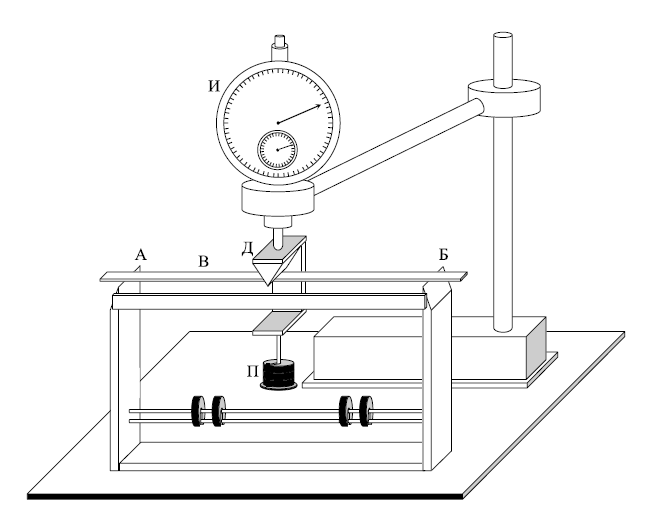
\includegraphics[width=\linewidth]{balka}
				\caption{Прибор для измерения модуля Юнга}
				\label{fig:balka}
			\end{minipage}\hfill
			\begin{minipage}{0.5\textwidth}
				\centering
				\begin{tikzpicture}[scale=1.25]
					\draw (0:0) -- (0:-1);
					\draw (0:0) -- (90:1);
					\draw[fill=white!90!black] (90:1) circle (0.2);
					
					\draw (0:0) -- (30:-1);
					\draw (0:0) -- (120:1);
					\draw[fill=white!90!black] (120:1) circle (0.2);
					
					\draw (-0.5,0) arc [radius=0.5, start angle=180, end angle=210];
					\draw (15:-0.7) node {$\alpha$};
					\draw[semithick,<->] (-1,-0.8) -- (0,-0.8);
					\draw (-0.5,-0.8) node[anchor=north] {$r$};
					\draw[semithick,<->] (0.3,0) -- (0.3,-0.6);
					\draw (0.3,-0.3) node[anchor=west] {$\Delta l$};
					
					\draw (-3.5, -4) rectangle (-3, 1.3);
					\foreach \x in {-3.5, -3.0, ..., 1.0} {
						\draw (-3.25,\x) -- (-3,\x);
					};
					\draw (-3,0.6) node[anchor=west] {$n_1$};
					\draw (-3,-3.6) node[anchor=west] {$n$};
					
					\draw[dashed] (-3,1) -- (0,1);
					\draw[dashed] (120:1) ++(-2.5,0) -- (120:1) -- ++(60:-5);
					\draw[dashed] (120:1) -- ++(30:-1);
					\draw[double] (120:1) ++(-0.5,0) arc [radius=0.5, start angle=180, end angle=240];
					\draw (120:1) ++(30:-1) node[fill=white] {$2\alpha$};
					
					\draw[semithick,<->] (0,-2.25) -- (-3,-2.25);
					\draw (-1.5,-2.25) node[anchor=north] {$h$};
				\end{tikzpicture}
				\caption{К нахождению $\Delta l$ по $n$}
				\label{fig:finddl}
			\end{minipage}
		\end{figure}
	\vspace{500px}

	\section{Ход работы}
		\subsection*{I часть}
			\begin{wraptable}{h}{6cm}
				\vspace{-0.5cm}
				\centering
				\caption*{\textbf{Параметры установки}}
				\vspace{-0.25cm}
				\begin{tabular}{cc}
					$d = 0.46 \text{ мм}$ & $l_0 = 176.8 \text{ см}$ \\
					$r = 15 \text{ cм}$ & $h = 133.4 \text{ см}$ \\
				\end{tabular}
			\end{wraptable}
	
			Получим формулу, связывающую удлинение проволоки $\Delta l$ с показаниями шкалы $n$. Из рисунка \ref{fig:finddl}:
			\[\tg\alpha = \frac{\Delta l}{r} \approx \alpha, \tg2\alpha = \frac{n - n_1}{h} \approx 2\alpha \Rightarrow \Delta l = \frac{r}{2h}\left(n - n_1\right)\]
			
			Оценим максимально допустимую нагрузку: при разрушающем напряжении $\sigma_{max} = 90 \frac{Ы\text{кг}}{\text{мм}^2}$ максимальная нагрузка составляет $0.3\sigma_{max}\pi \frac{d^2}{4} \approx 45 \text{ Н}$.
			
			Снимем зависимость удлинения проволоки от массы грузов, трижды увеличивая и уменьшая нагрузку на проволоку, и занесём результат в таблицу \ref{table:n(m)}.
					
			\begin{table}[h]
				\caption{Зависимость показаний $n$ шкалы от нагрузки $m$.}
				\label{table:n(m)}
				\begin{tabular}{|c|r|r|r|r|r|r||r|r|r|r|r|r|}
					\hline
					$m$, г & $455.3$ & $700.1$ & $946.2$ & $1191.9$ & $1437.5$ & $1928.4$ & $1682.8$ & $1437.5$ & $1191.9$ & $946.2$ & $700.1$ \\
					\hline
					$n$, см & $12.2$ & $14.9$ & $17.7$ & $20.3$ & $22.8$ & $27.6$ & $25.2$ & $22.7$ & $20.1$ & $17.6$ & $14.8$ \\
					\hline \hline
					$m$, г & $946.2$ & $1437.5$ & $1928.4$ & $2173.9$ & $2419.1$ & $2664.7$ & $2419.1$ & $2173.9$ & $1682.8$ & $1191.9$ & $946.2$ \\
					\hline
					$n$, см & $17.8$ & $22.7$ & $27.6$ & $29.9$ & $31.8$ & $34.5$ & $32.2$ & $29.9$ & $25.2$ & $20.4$ & $17.8$ \\
					\hline \hline
					$m$, г & $1191.9$ & $1682.8$ & $2173.9$ & $2419.1$ & $2664.7$ & $3154.6$ & $2909.1$ & $2419.1$ & $2173.9$ & $1682.8$ & $1191.9$ \\
					\hline
					$n$, см & $20.3$ & $25.2$ & $29.9$ & $32.2$ & $34.6$ & $39.2$ & $37.0$ & $32.4$ & $30.0$ & $25.2$ & $20.3$ \\
					\hline
				\end{tabular}
			\end{table}
			
			Отметим, что начальное показание шкалы $n_0 \neq 0$, так что в данном случае закон Гука принимает следующий вид:
			\[P^\ast = (m + m_0)g = k (l - l_0) = k \left(l - l_1 - \left(l_0 - l_1\right)\right) = k (\Delta l - \Delta l_1) \Rightarrow mg = k\frac{r}{2h}(n - n_1) + const\]
			В итоге получаем зависимость $n(m)$:
			\[n = \frac{1}{k^\ast} m + const \text{, где } \frac{1}{k^\ast} = \frac1k \frac{2hg}{r}\]
			Построим график этой зависимости (рис. \ref{fig:first_part}) и по методу наименьших квадратов оценим параметр $k$. Будем принимать во внимание тот факт, что при малых нагрузках проволока только распрямляется и линейный закон Гука не выполняется --- учитывать в расчётах измерения с массами меньше 900 грамм не будем.
			\newpage
			\begin{figure}[t]
				\centering
				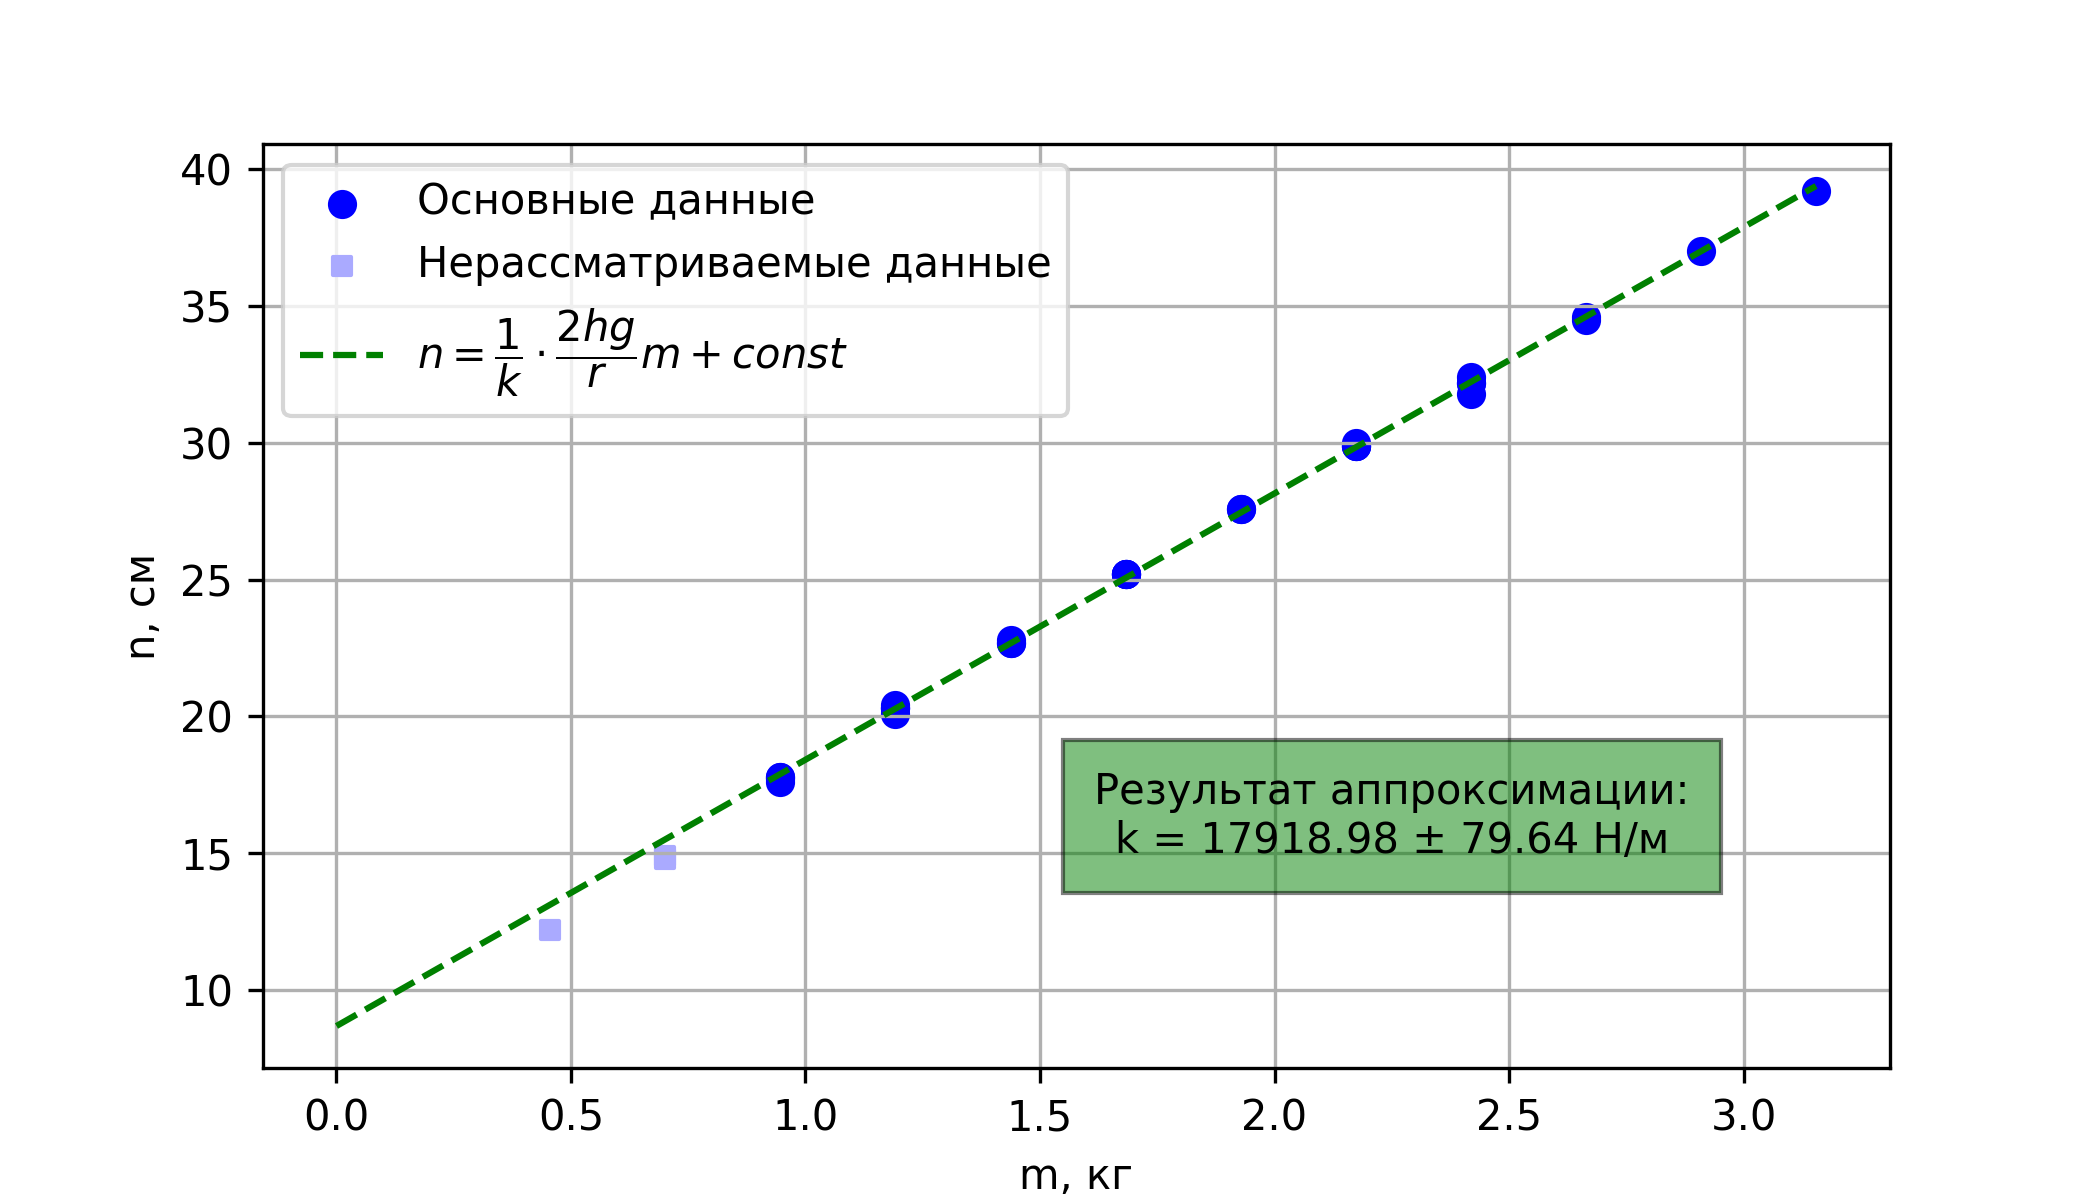
\includegraphics[width=\linewidth]{first_part}
				\caption{Зависимость показаний шкалы от массы грузов}
				\label{fig:first_part}
			\end{figure}
		
			Оценим систематическую ошибку измерения упругости проволоки:
			\[\frac{{\Delta_k}^2}{k^2} = \frac{\Delta_n^2}{n^2} + \frac{\Delta_h^2}{h^2} = 0.01^2 + 0.004^2 \approx 0.01^2\]
			
			Полная погрешность составляет:
			\[\sigma_k = \sqrt{\Delta_k^2 + {\sigma_k^\text{случ}}^2} = \sqrt{\left(17919 \cdot 0.01\right)^2 + 79.64^2} = 196.1 \text{ Н $\cdot$ м$^{-1}$}\]
			
			Модуль Юнга и погрешность его измерения находим по формулам:
			\[E = \frac{4kl_0}{\pi d^2} = 19.06 \times 10^{10} \text{ Н $\cdot$ м$^{-2}$}\]
			\[\sigma_E= E\sqrt{{\epsilon_{l_0}}^2 + \epsilon_d^2 + \epsilon_k^2} = E\sqrt{\left(\frac{0.05}{176.8}\right)^2 + \left(2 \cdot \frac{0.005}{0.46}\right)^2 + \left(\frac{\sigma_k}{k}\right)^2} = 4.64\times10^9 \text{ Н $\cdot$ м$^{-2}$}\]
			
			Полученное в ходе эксперимента значение \fbox{$E = (19.06 \pm 0.46) \times 10^{10}$ Па} соответствует табличному значению модуля Юнга \textit{железа}.

		\subsection*{II часть}
			\begin{wraptable}{h}{6cm}
				\vspace{-0.5cm}
				\centering
				\caption*{\textbf{Параметры установки}}
				\vspace{-0.25cm}
				\begin{tabular}{cc}
					$l = 503 \text{ мм}$ & $m_0 = 54.5 \text{ г}$ \\
				\end{tabular}
			\end{wraptable}
			
			Измерим размеры каждой балки в десяти местах, данные отражены в таблице \ref{table:rods}. Средние значения размеров балок и их погрешности представлены в той же таблице, при этом мы воспользовались следующими формулами:
			\[\mean{d} = \frac{\sum d_i}{N} \hspace{1cm} \sigma_d = \sqrt{\frac{\sum{\left( d_i - \mean{d}\right)^2}}{N - 1}} \hspace{1cm} \sigma_{\mean{d}} = \frac{\sigma_d}{\sqrt{N}} \hspace{1cm} \sigma_\text{полн} = \sqrt{{\sigma_{\mean d}}^2 + {\Delta_d}^2} \]
		
			\begin{table}[t]
				\centering
				\caption{Измерения размеров балок}
				\label{table:rods}
				\makebox[\textwidth][c]{
				\begin{tabular}{|c|c|r|r|r|r|r|r|r|r|r|r||c|}
					\hline
					\multirow{2}{*}{металл} & a, мм & 21.5 & 21.3 & 21.0 & 20.9 & 21.2 & 21.4 & 21.2 & 21.0 & 21.3 & 21.2 & $21.20 \pm 0.1$ мм \\
					\hhline{|~|-|-|-|-|-|-|-|-|-|-|-||-|}
					& b, мм & 3.81 & 3.8 & 3.81 & 3.87 & 3.87 & 3.83 & 3.85 & 3.8 & 3.81 & 3.87 & $3.83 \pm 0.01$ мм\\
					\hhline{=============}
					\multirow{2}{*}{латунь} & a, мм & 21.5 & 21.5 & 21.4 & 21.6 & 21.4 & 21.5 & 21.5 & 21.5 & 21.5 & 21.4 & $21.5 \pm 0.1$ мм \\
					\hhline{|~|-|-|-|-|-|-|-|-|-|-|-||-|}
					& b, мм & 3.92 & 3.92 & 3.93 & 3.93 & 3.92 & 3.92 & 3.93 & 3.91 & 3.93 & 3.92 & $3.92 \pm 0.01$ мм \\
					\hhline{=============}
					\multirow{2}{*}{дерево} & a, мм & 19.3 & 19.1 & 19.2 & 19.2 & 19.1 & 19.3 & 19.3 & 19.1 & 19.3 & 19.3 & $19.2 \pm 0.1$ мм \\
					\hhline{|~|-|-|-|-|-|-|-|-|-|-|-||-|}
					& b, мм & 10.31 & 10.19 & 10.22 & 10.31 & 10.23 & 10.17 & 10.2 & 10.16 & 10.31 & 10.18 & $10.29 \pm 0.02$ мм \\
					\hline
				\end{tabular}
				}
			\end{table}

		\begin{table}
			\caption{Измерения стрелы прогиба металлической балки}
			\label{table:metal}
			\makebox[\textwidth][c]{
			\begin{tabular}{|c|c|r|r|r|r|r|r|r|r|r|r|r|}
				\hline
				\multirow{2}{1cm}{\centering непер.} & $m$, г & 559.0 & 1056.2 & 1564.9 & 2066.9 & 2566.9 & 3069.9 & 2566.9 & 2066.9 & 1564.9 & 1056.2 & 559.0 \\
				\hhline{|~|-|-|-|-|-|-|-|-|-|-|-|-|}
				& $y_{max}$, мм & 0.68 & 1.36 & 2.06 & 2.75 & 3.44 & 4.14 & 3.45 & 2.77 & 2.07 & 1.38 & 0.7 \\
				\hhline{=============}
				\multirow{2}{1cm}{\centering пер.} & $m$, г & 559.0 & 1067.7 & 1570.7 & 2066.9 & 2570.4 & 2067.6 & 2574.4 & 2066.9 & 1570.7 & 1067.7 & 559.0 \\
				\hhline{|~|-|-|-|-|-|-|-|-|-|-|-|-|}
				& $y_{max}$, мм & 0.68 & 1.38 & 2.09 & 2.78 & 3.48 & 4.18 & 3.52 & 2.82 & 2.15 & 1.47 & 0.76 \\
				\hhline{=============}
				\multirow{2}{1cm}{\centering смещ. непер.} & $m$, г & 551.7 & 1056.2 & 1559.2 & 2061.2 & 2557.4 & 3060.9 & 2557.4 & 2061.2 & 1559.2 & 1056.2 & 551.7 \\
				\hhline{|~|-|-|-|-|-|-|-|-|-|-|-|-|}
				& $y_{max}$, мм & 0.66 & 1.4 & 2.08 & 2.79 & 3.47 & 4.19 & 3.51 & 2.83 & 2.14 & 1.45 & 0.74 \\
				\hhline{=============}
				\multirow{2}{1cm}{\centering смещ. пер.} & $m$, г & 551.7 & 1056.2 & 1559.2 & 2061.2 & 2557.4 & 3060.9 & 2557.4 & 2061.2 & 1559.2 & 1056.2 & 551.7 \\
				\hhline{|~|-|-|-|-|-|-|-|-|-|-|-|-|}
				& $y_{max}$, мм & 0.7 & 1.41 & 2.11 & 2.83 & 3.5 & 4.24 & 3.56 & 2.89 & 2.18 & 1.5 & 0.81 \\
				\hline
			\end{tabular}
			}
		\end{table}
		
		\begin{table}
			\centering
			\caption{Измерения стрелы прогиба латунной балки}
			\label{table:brass}
			\makebox[\textwidth][c]{
			\begin{tabular}{|c|c|r|r|r|r|r|r|r|r|r|}
				\hline
				\multirow{2}{1cm}{\centering непер.} & $m$, г & 551.7 & 1056.2 & 1559.2 & 2055.4 & 2557.4 & 2055.4 & 1559.2 & 1056.2 & 551.7 \\
				\hhline{|~|-|-|-|-|-|-|-|-|-|-|}
				& $y_{max}$, мм & 1.2 & 2.45 & 3.71 & 4.91 & 6.15 & 4.95 & 3.72 & 2.47 & 1.23 \\
				\hhline{===========}
				\multirow{2}{1cm}{\centering пер.} & $m$, г & 551.7 & 1056.2 & 1559.2 & 2055.4 & 2557.4 & 2055.4 & 1559.2 & 1056.2 & 551.7 \\
				\hhline{|~|-|-|-|-|-|-|-|-|-|-|}
				& $y_{max}$, мм & 1.14 & 2.42 & 3.64 & 4.84 & 6.06 & 4.86 & 3.67 & 2.49 & 1.25 \\
				\hline
			\end{tabular}
			}
		\end{table}
		
		\begin{table}
			\centering
			\caption{Измерения стрелы прогиба деревянной балки}
			\label{table:wood}
			\makebox[\textwidth][c]{
			\begin{tabular}{|c|c|r|r|r|r|r|r|r|r|r|r|r|}
				\hline
				\multirow{2}{1cm}{\centering непер.} & $m$, г & 551.7 & 1056.2 & 1559.2 & 2055.4 & 2557.4 & 3060.9 & 2557.4 & 2055.4 & 1559.2 & 1056.2 & 551.7 \\
				\hhline{|~|-|-|-|-|-|-|-|-|-|-|-|-|}
				& $y_{max}$, мм & 0.57 & 1.18 & 1.78 & 2.37 & 2.97 & 3.55 & 3.0 & 2.42 & 1.84 & 1.26 & 0.67 \\
				\hhline{=============}
				\multirow{2}{1cm}{\centering пер.} & $m$, г & 551.7 & 1056.2 & 1559.2 & 2055.4 & 2557.4 & 3060.9 & 2557.4 & 2055.4 & 1559.2 & 1056.2 & 551.7 \\
				\hhline{|~|-|-|-|-|-|-|-|-|-|-|-|-|}
				& $y_{max}$, мм & 0.61 & 1.24 & 1.85 & 2.43 & 3.06 & 3.65 & 3.1 & 2.5 & 1.91 & 1.3 & 0.69 \\
				\hline
			\end{tabular}
			}
		\end{table}

\end{document}